\section{Literaturbeispiele} % (fold)
\label{sec:literaturbeispiele}

	\begin{figure}[H]
		\center
		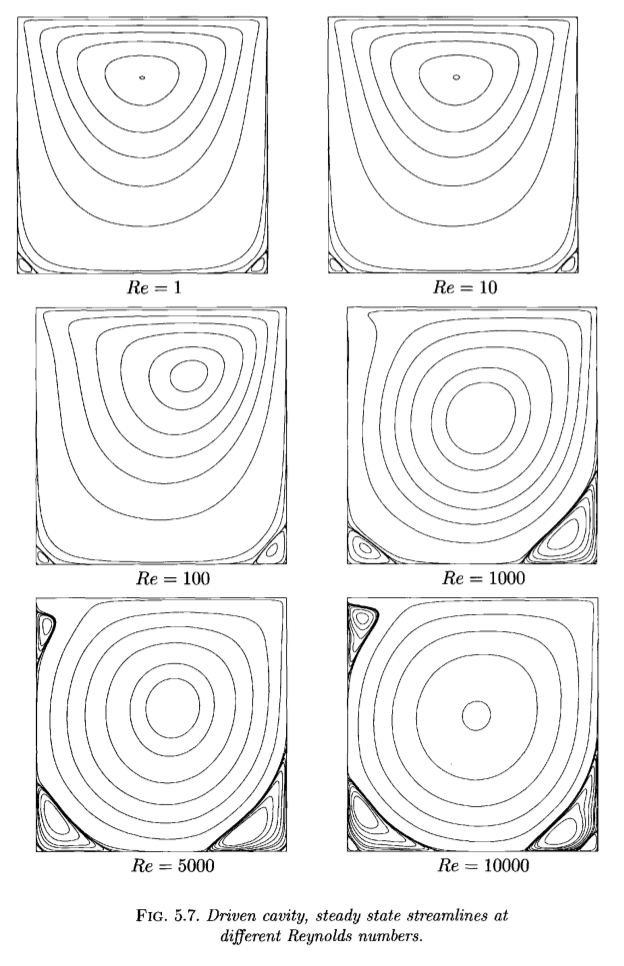
\includegraphics[scale = 0.5]{screenshots/literatur-re-01.png}
		\caption{Simulation des stationären Geschwindigkeitsfeldes für verschiedene Reynoldszahlen \\ Quelle: \cite{nsfd} }
		\label{fig:literatur re 01}
	\end{figure}

	% \begin{figure}[H]
	% 	\center
	% 	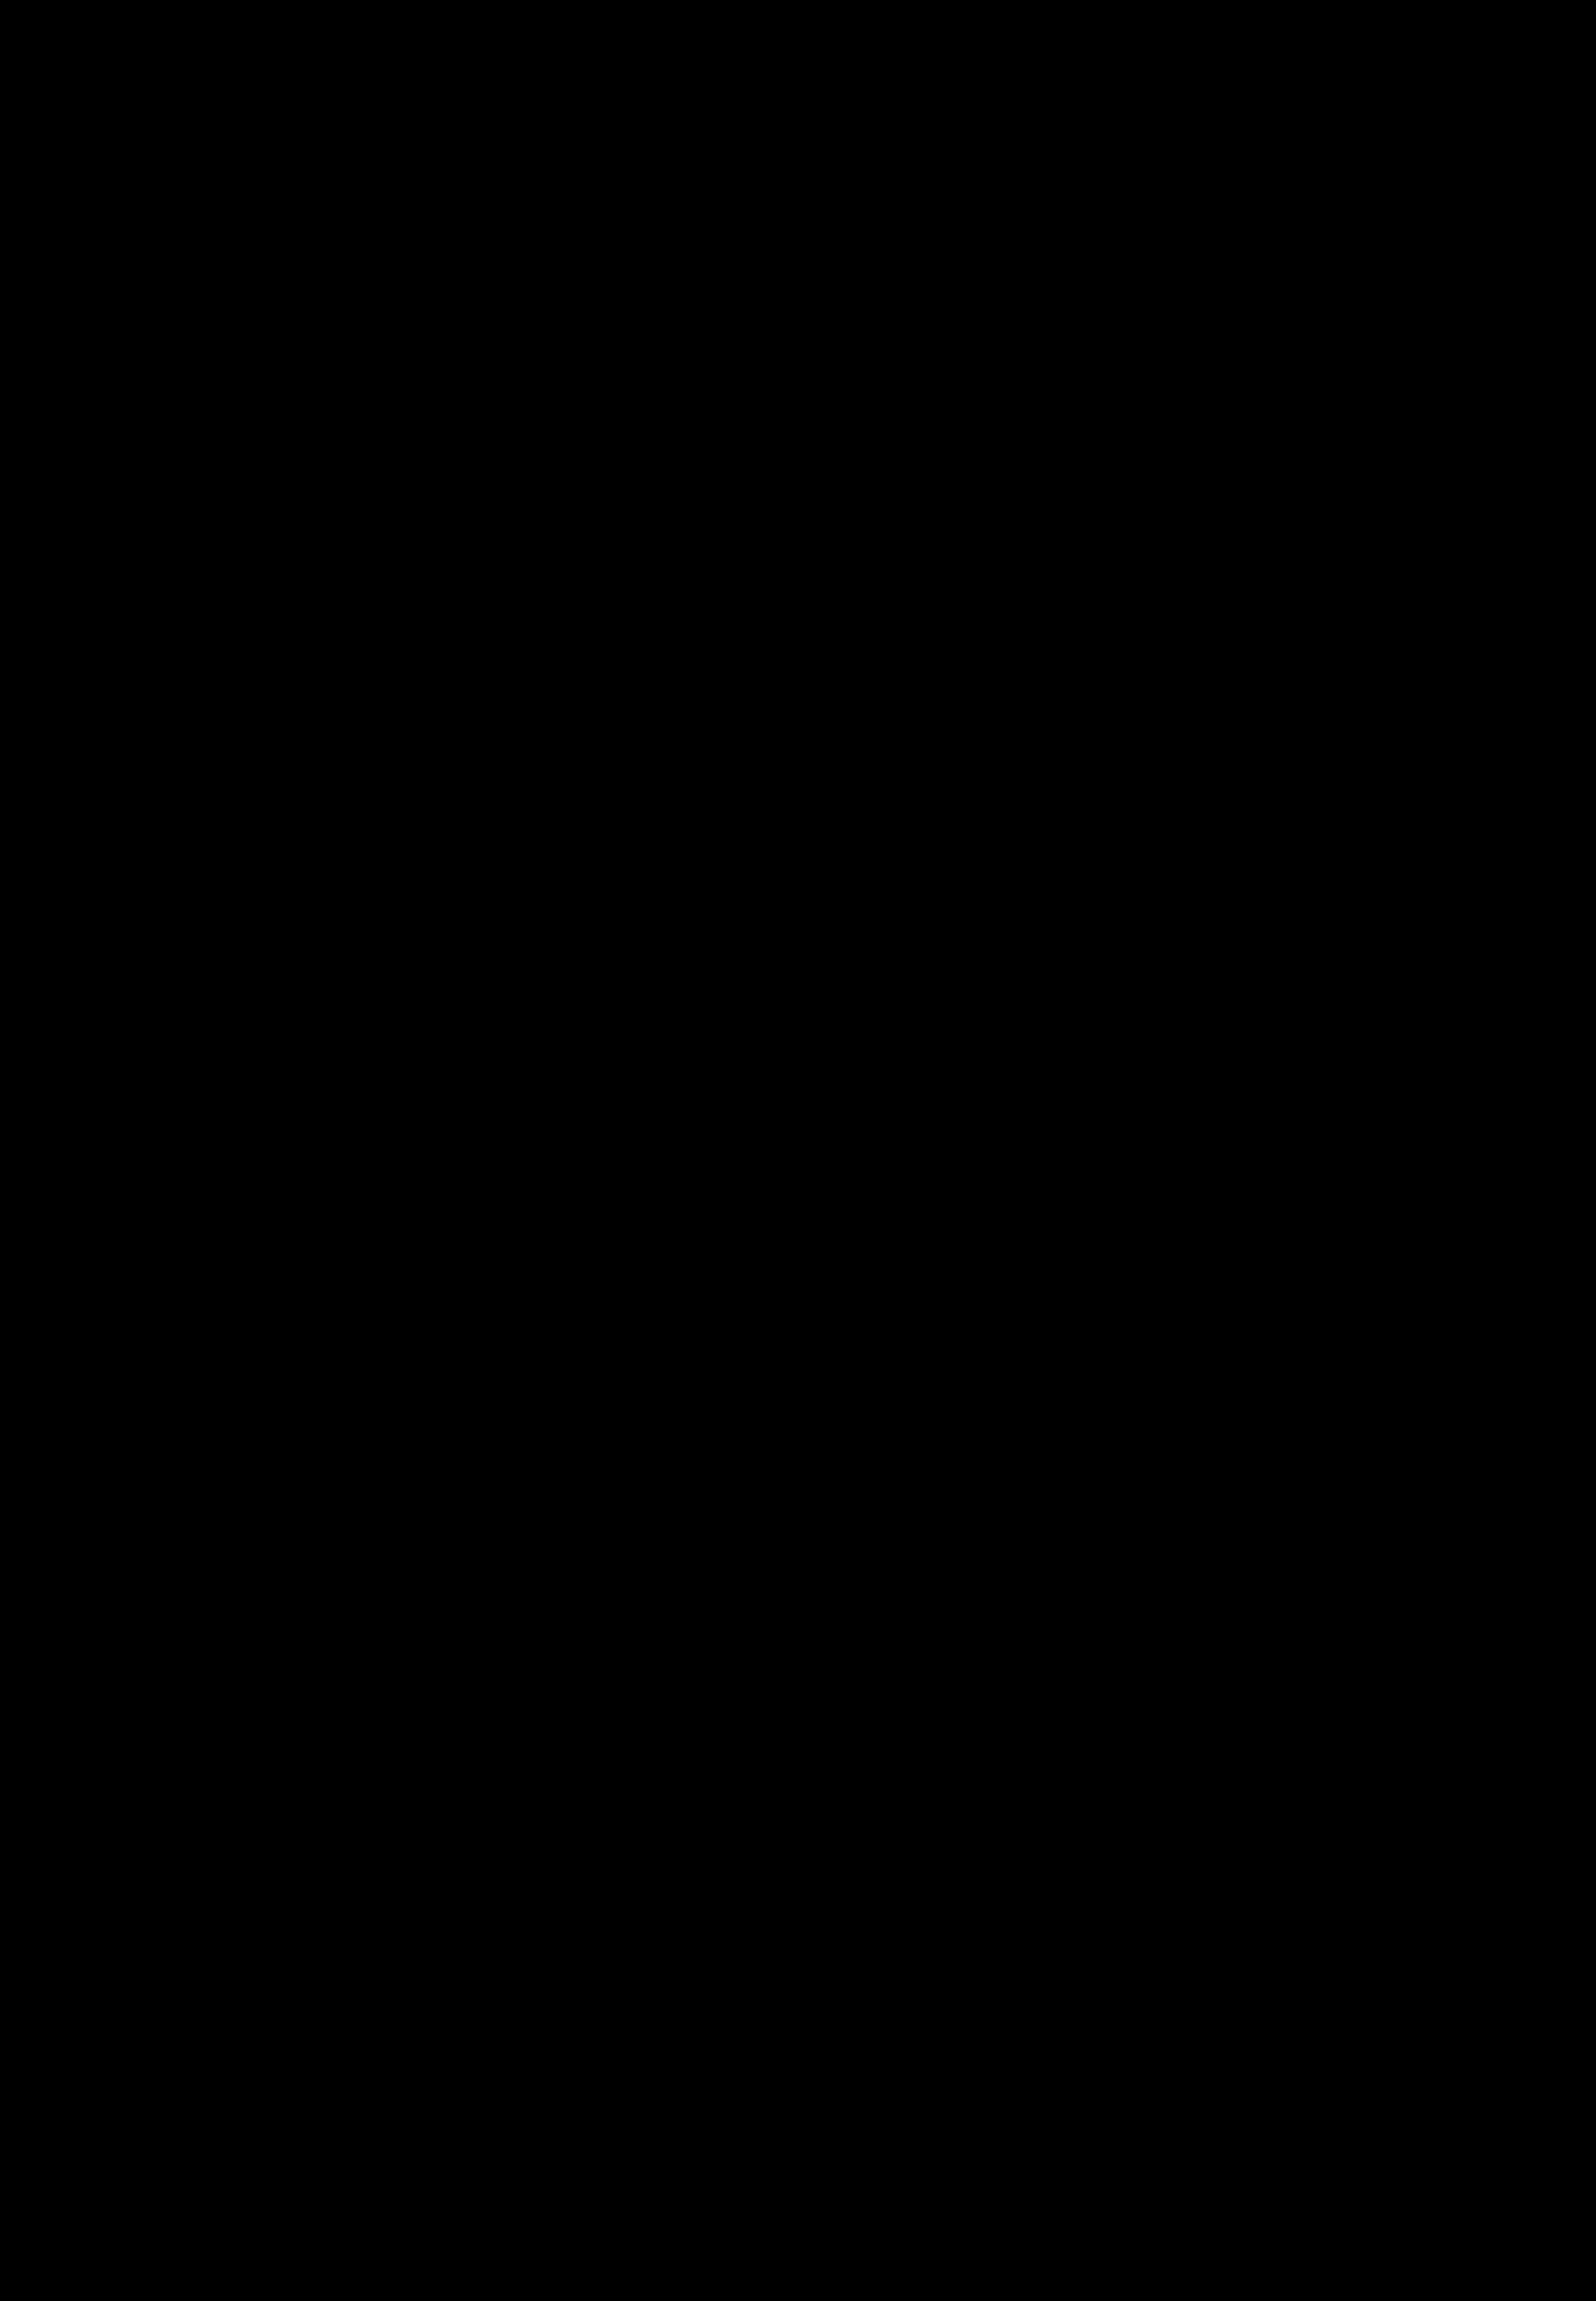
\includegraphics[scale = 0.5]{screenshots/literatur-re-02.png}
	% 	\caption{}
	% 	\label{fig:literatur re 02}
	% \end{figure}

	\begin{figure}[H]
		\center
		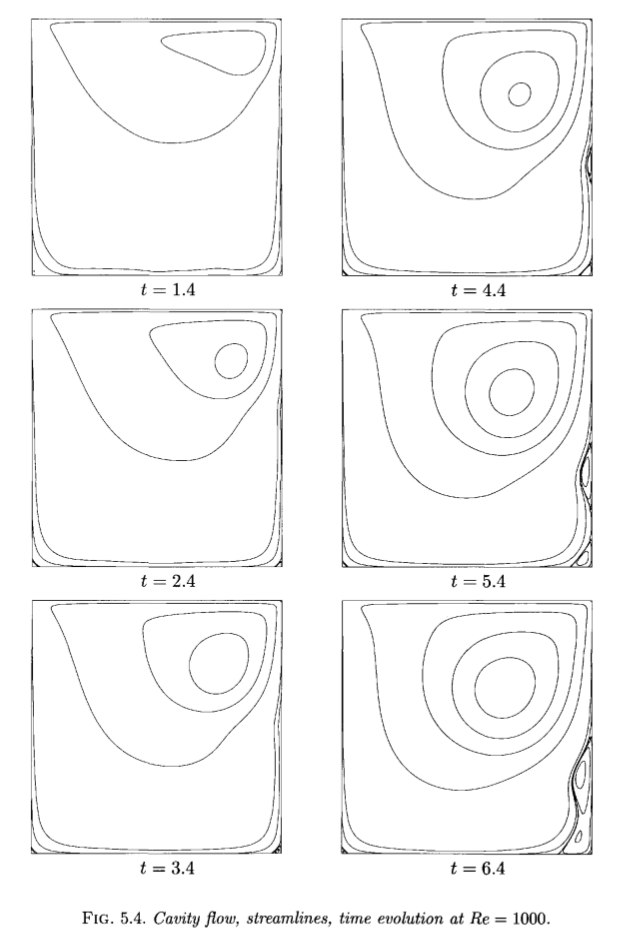
\includegraphics[scale = 0.5]{screenshots/literatur-time-01.png}
		\caption{Zeitevolution des Geschwindigkeitsfeldes für $Re=1000$ \\ Quelle: \cite{nsfd} }
		\label{fig:literatur time 01}
	\end{figure}

	\begin{figure}[H]
		\center
		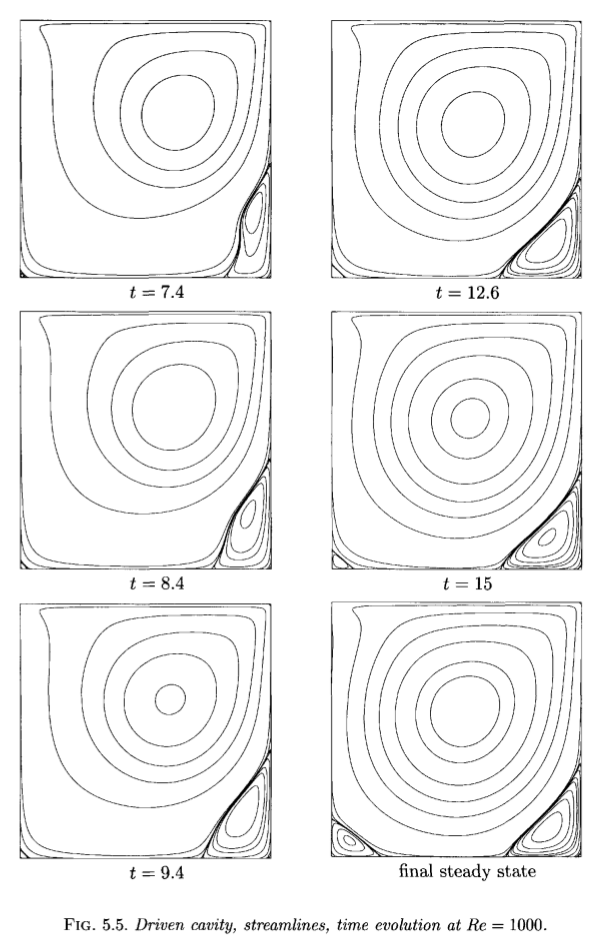
\includegraphics[scale = 0.5]{screenshots/literatur-time-02.png}
		\caption{Zeitevolution des Geschwindigkeitsfeldes für $Re=1000$ \\ Quelle: \cite{nsfd} }
		\label{fig:literatur time 02}
	\end{figure}


% section literaturbeispiele (end)